\documentclass[crop,tikz,border=2px]{standalone}
\usepackage{tikzsymbols}
\usetikzlibrary{calc,arrows,positioning}
\begin{document}
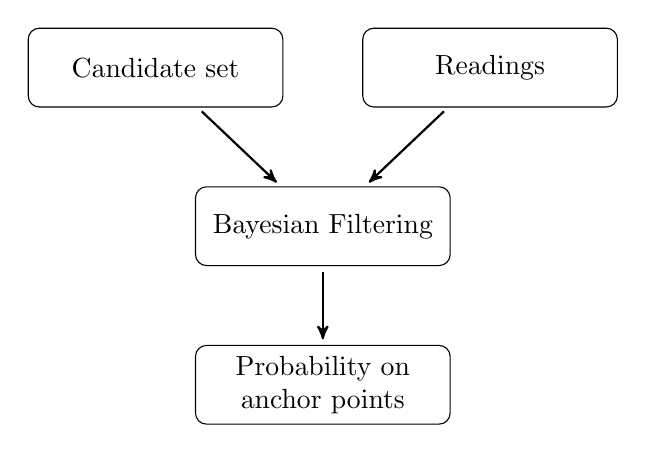
\begin{tikzpicture}[remember picture,
  myrect/.style={draw,rounded corners,rectangle,text width=3cm,text
    centered,minimum height=1cm},
  arrow/.style={->,>=stealth',thick,shorten <=2pt,shorten >=2pt}]

  \node[myrect] (i0) {Candidate set};
  \node[myrect] (i1) [right=of i0] {Readings};
  \coordinate (mid) at ($(i0.south)!0.5!(i1.south)$);
  \node[myrect] (filter) [below=of mid] {Bayesian Filtering};
  \node[myrect] (out) [below=of filter] {Probability on anchor points};

  \draw[arrow] (i0) -- (filter);
  \draw[arrow] (i1) -- (filter);
  \draw[arrow] (filter) -- (out);
\end{tikzpicture}
\end{document}